\section{Tahapan Cara Membuat Aplikasi}
Berikut Adalah Tahapan Cara membuat aplikasi, dengan menuju halaman utama aplikasi Oracle APEX anda akan mendapati App Builder yang berfungsi untuk membuat aplikasi WEB atau disebut Web Based Application dengan perantara host yang disediakan oleh Oracle APEX.

\par pada saat membuat aplikasi web caranya sangat mudah seperti kita hanya akan mendrag dan drop, namun ada juga yang harus pakai koding html/css untuk menambah fitur lainnya, langsung saja cek di bawah ini.
   
\begin{itemize}
        \begin{figure}[!htbp]
        \item[1]Pilih Create App.
        \begin{center}
        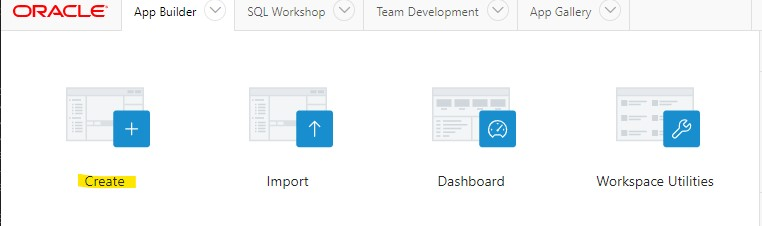
\includegraphics[scale=0.4]{figures/create_app.jpg}
        \caption{\textit{Create App}}
        \end{center}
        \par Pada tahapan ini anda akan diberikan 4 pilihan yaitu :
        \begin{itemize}
            \item Create = Untuk membuat Aplikasi (Pilih yang ini)
            \item Import = Untuk mengimpor aplikasi yang sudah ada/jadi
            \item Dashboard = melihat dasbor aplikasi yang sudah ada
            \item Workspace Utilities = Utiliti Workspace
        \end{itemize}
        \end{figure}
        
        \begin{figure}[!htbp]
        \item[2]Pilih New Application 
        \begin{center}
        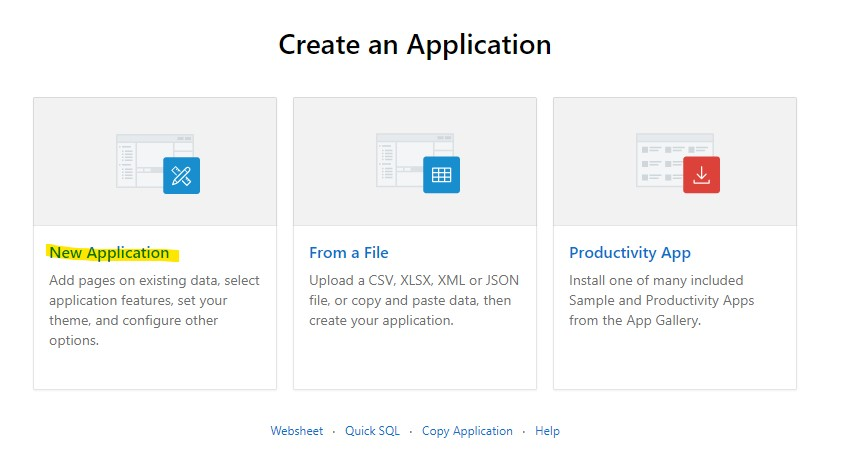
\includegraphics[scale=0.5]{figures/create_a_new_application.jpg}
        \caption{\textit{Pilih New Application}}
        \end{center}
        \par Berikut adalah tahapan membuat aplikasi, anda akan diberikan 3 pilihan yaitu :
            \begin{itemize}
                \item New Application = Untuk membuat halaman aplikasi baru yang sudah ada data tabel yang telah diinputkan pada sql query (Pilih yang ini).
                \item From a File = Membuat aplikasi dari data yang sudah ada namun menggunakan file Excell/XLSX/JSON.
                \item Productivity App = Install aplikasi yang sudah ada dalam Oracle Apex dari App Galery.
            \end{itemize}
        \end{figure}
        
        \begin{figure}[!htbp]
        \item[3]Klik Add Page
        \begin{center}
        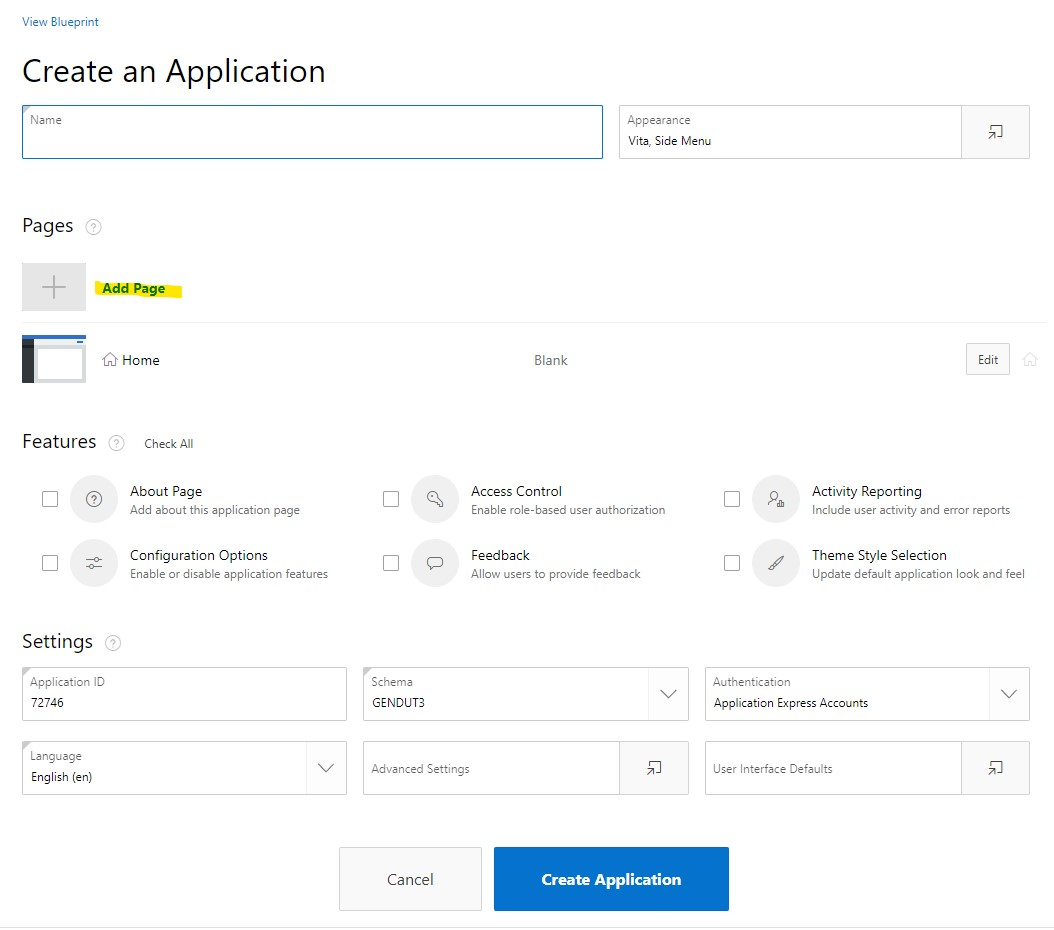
\includegraphics[scale=0.4]{figures/klik_add_page.jpg}
        \caption{\textit{Klik Add Page}}
        \end{center}
        \begin{itemize}
            \item Untuk menambahkan page klik di kolom page, lalu pilih tampilan. Untuk page pertama yaitu query tabel Data Staf, pastikan kalian pilih tampilan sebagai Interactive Report. Lalu masukan nama pagenya setelah itu arahkan ke tabel mana page Interactive Report tersebut. Karena kita ingin melakukan query terhadap tabel Data Staf, maka kita isikan tabelnya adalah Data Staf. 
        \end{itemize}
        \end{figure}
        
        \begin{figure}[!htbp]
        \item[4]Berikut adalah pilihan dari fungsi add page
        \begin{center}
        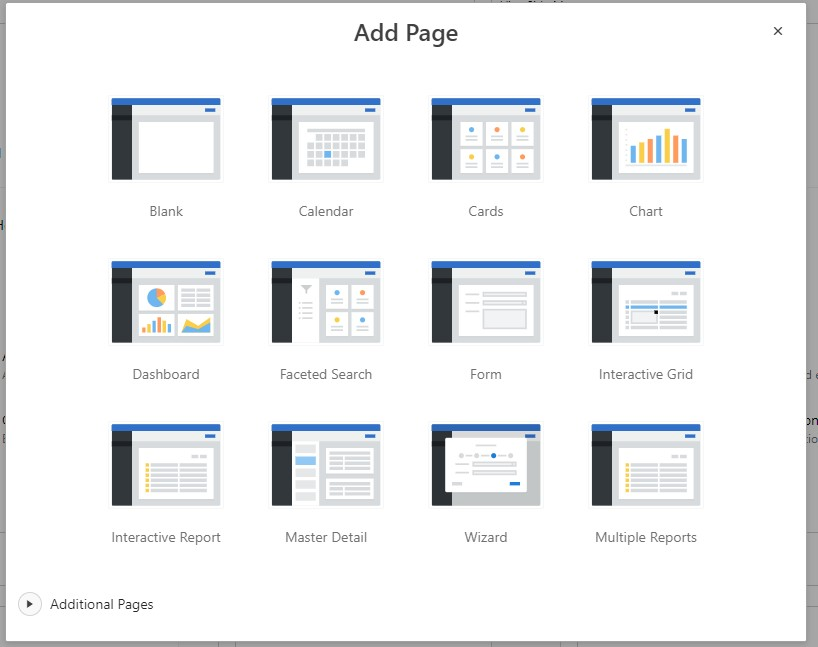
\includegraphics[scale=0.4]{figures/fungsi_add_page.jpg}
        \caption{\textit{Pilihan dari fungsi add page}}
        \end{center}
        \begin{itemize}
            \item Blank = Adalah page yang tidak berisi anda bebas untuk mengisi perlengkapannya seperti item tombol-tombol saat membuat page ini.
            \item Calender = Adalah Page yang berfungsi untuk menambahkan kalender yang di ambil datanya dari database.
            \item Cards = Adalah page yang berisi navigasi untuk membuat item beserta data dari beberapa database.
            \item Charts = Adalah Page yang berisi Laporan yang terstruktur dengan menggunakan chart yang mengambil datanya dari database.
            \item Dashboard = Adalah Page navigasi antara Page atau untuk menampilkan beberapa data atau laporan.
            \item Faceted Search = Adalah Page yang berfungsi untuk search dari Page Lainnya.
            \item Form = Adalah page yang brfungsi untuk membuat form yang nanti akan terisi ke database.
            \item Interactive Grid = Adalah tampilan laporan data dari database.
            \item Interractive Report = Adalah Page untuk menampilkan laporan data yang dapat di edit serta menampilkan hanya beberapa data saja.
            \item Master Detail = Adalah Page yang berfungsi menampilkan data dari database yang telah ternormalisasi seperti relasi antar tabel.
            \item Wizard = Adalah Page untuk menampilkan Form seperti Massage Box atau alert.
            \item Multiple Report = Adalah Page yang berfungsu melihat beberapa report dari tabel database.
        \end{itemize}
        \end{figure}
        
        \begin{figure}[!htbp]
        
        \item[5]Silahkan Pilih Interractive Report
        \begin{center}
        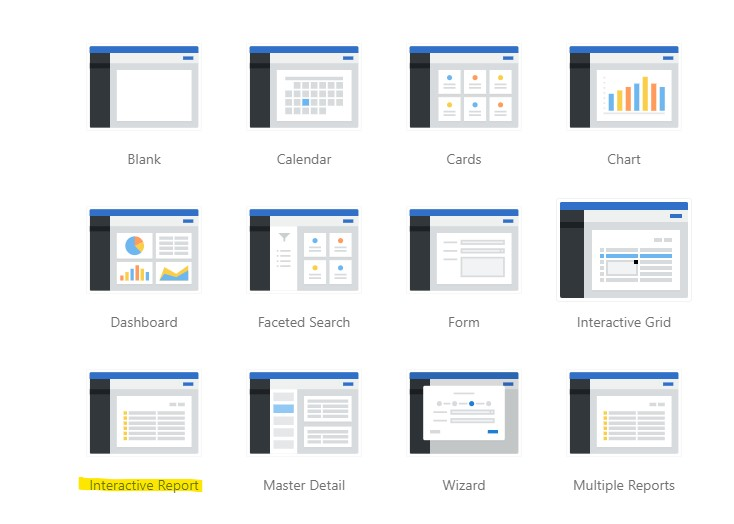
\includegraphics[scale=0.6]{figures/pilih_interractive_report.jpg}
        \caption{\textit{Memilih Interactive Report}}
        \end{center}
                \begin{itemize}
            \item Pilih Interractive Report , mengapa interractive report , agar data dari tabel bisa terstruktur dan  dapat di edit secara langsung dan dapat menampilkan hanya beberapa data yang dibutuhkan
        \end{itemize}
        \end{figure}
        
        \begin{figure}[!htbp]
        \item[6]Anda akan dialihkan ke Add Page Report
        \begin{center}
        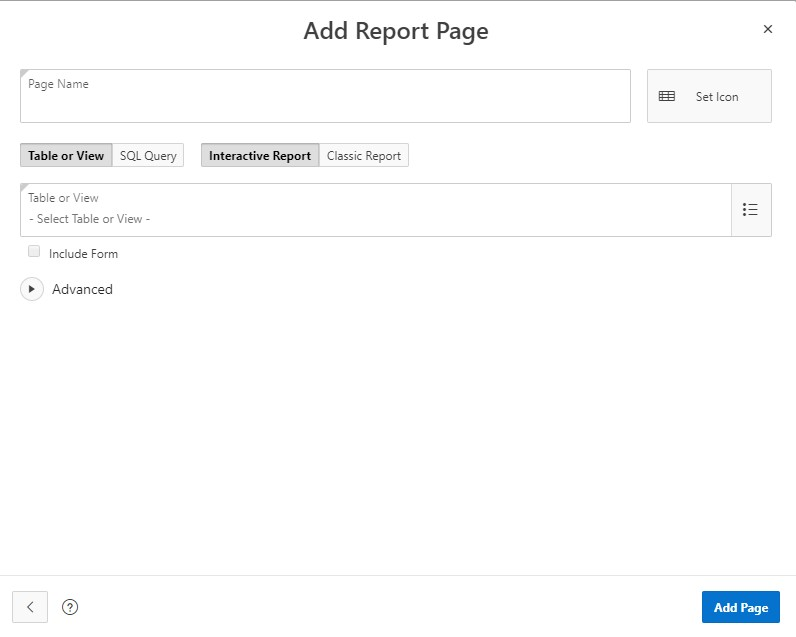
\includegraphics[scale=0.5]{figures/menambahkan_page_report.jpg}
        \caption{\textit{Add Report Page}}
        \end{center}
        \begin{itemize}
            \item Table untuk mengisi kolom yang sudah kita buat tadi
        \end{itemize}
        \end{figure}
        
        \begin{figure}[!htbp]
        \item[7]Ikuti cara berikut kita akan membuat Report Page Beserta Form dari tabel Mahasiswa
        \begin{center}
        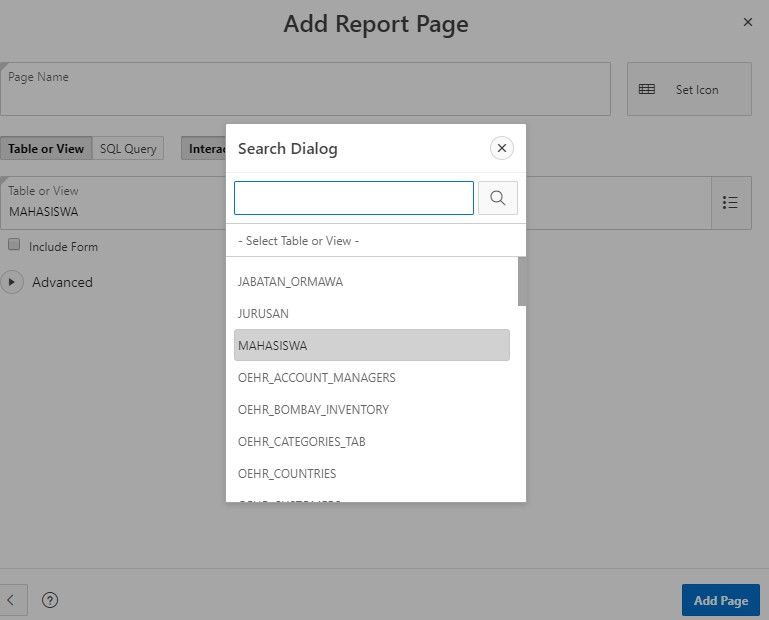
\includegraphics[scale=0.5]{figures/ambil_database_mahasiswa.jpg}
        \caption{\textit{Memilih Tabel Mahasiswa}}
        \end{center}
        \begin{itemize}
            \item Pilih nama mana yang mau anda masukan duluan 
        \end{itemize}
        \end{figure}
        
        \begin{figure}[!htbp]
        \item[8]Lengkapi isian interactive report berikut 
        \begin{center}
        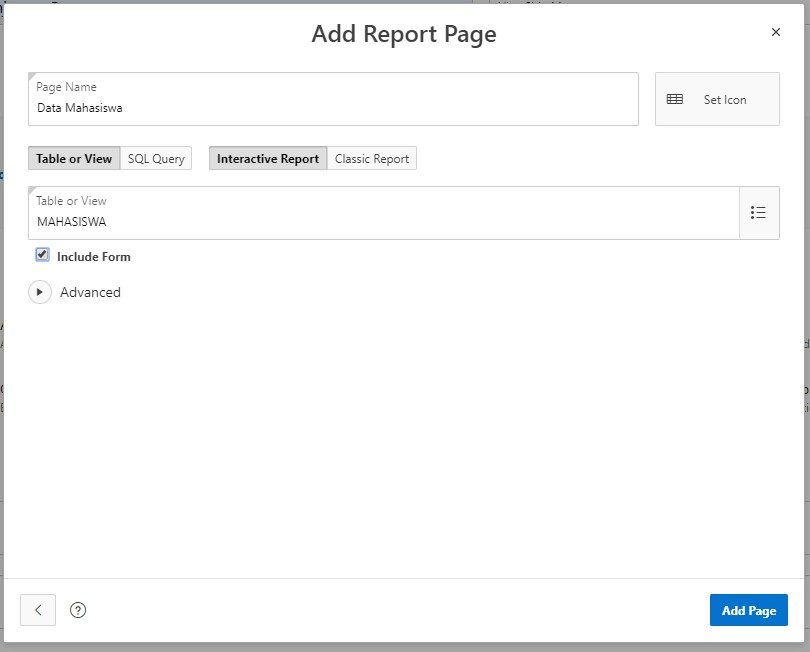
\includegraphics[scale=0.5]{figures/lengkapi_form_interractive.jpg}
        \caption{\textit{Melengkapi Isian Form Interractive}}
        \end{center}
        \begin{itemize}
            \item Pastikan terisi semuanya lalu klik add page  
        \end{itemize}
        \end{figure}
        
        \begin{figure}[!htbp]
        \item[9]Ubah Logo Ikon Pada Page
        \begin{center}
        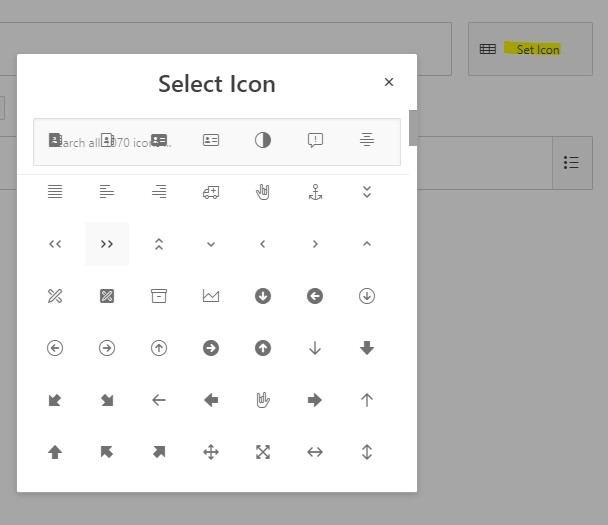
\includegraphics[scale=0.5]{figures/set_icon_interractive.jpg}
        \caption{\textit{Set Icon Page}}
        \end{center}
        \begin{itemize}
            \item pilih ikon yang menurut anda cocok untuk icon table
        \end{itemize}
        \end{figure}
        
        \begin{figure}[!htbp]
        \item[10]Klik Add Page
        \begin{center}
        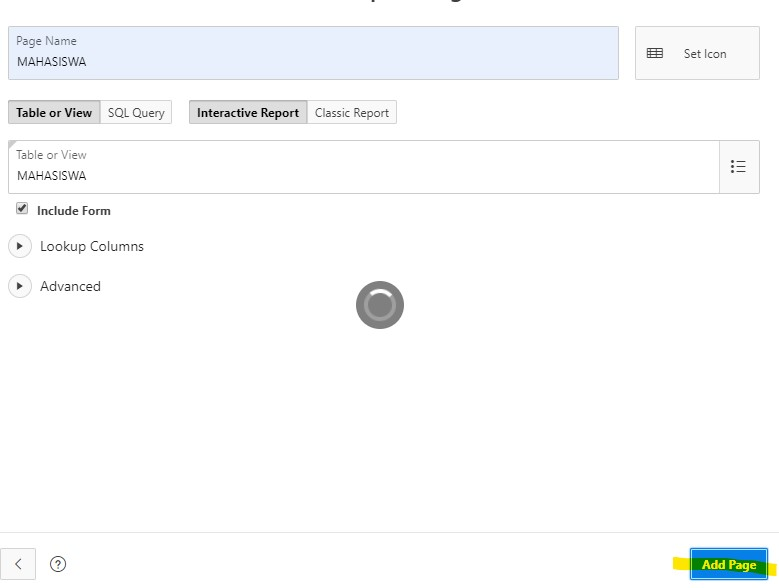
\includegraphics[scale=0.5]{figures/klick_add_page.jpg}
        \caption{\textit{Add Page}}
        \end{center}
       \begin{itemize}
            \item Kalau semua sudah terisi dengan benar lalu add page 
        \end{itemize}
        \end{figure}
        
        \begin{figure}[!htbp]
        \item[11]Untuk Melengkapi Admin silahkan centang features admin berikut
        \begin{center}
        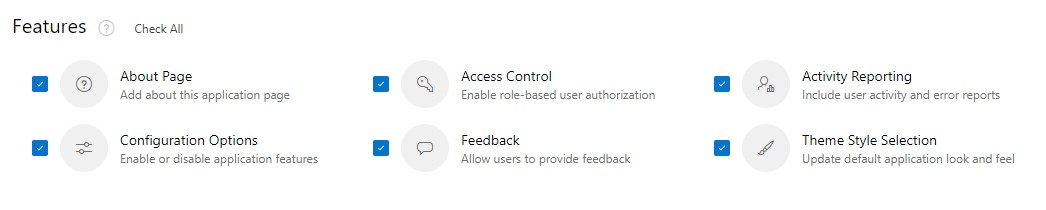
\includegraphics[scale=0.4]{figures/untuk_lengkapi_admin.jpg}
        \caption{\textit{Untuk Melengkapi Admin}}
        \end{center}
        \begin{itemize}
            \item Centang semua FEATURES nya untuk menampilkan pengaturan di aplikasinya 
        \end{itemize}
        \end{figure}
        
        \begin{figure}[!htbp]
        \item[12]Berikut adalah Appearance untuk mengganti tema utama pada aplikasi anda
        \begin{center}
        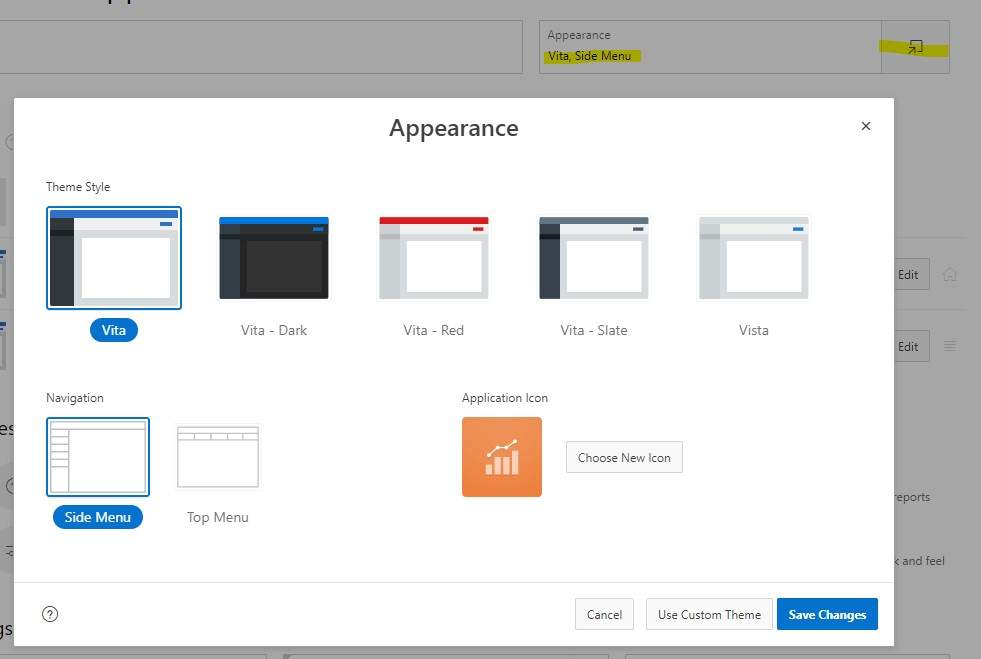
\includegraphics[scale=0.4]{figures/untuk_mengganti_tema.jpg}
        \caption{\textit{Mengganti Tema}}
        \end{center}
        \begin{itemize}
            \item Pilih tema yang menurut anda bagus lalu klik
        \end{itemize}
        \end{figure}
        
        \begin{figure}[!htbp]
        \item[13]Lalu klik Save Changes setelah mengganti tema
        \begin{center}
        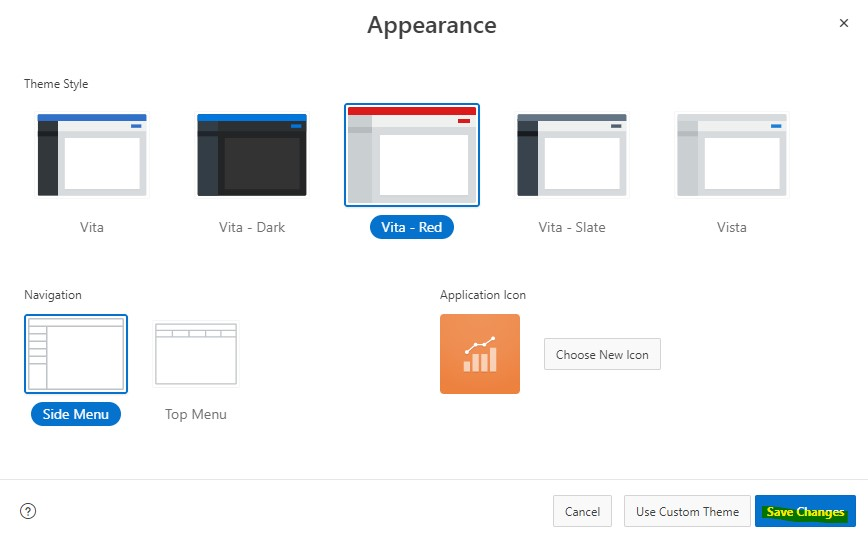
\includegraphics[scale=0.4]{figures/pilih_tema_lalu_klik_save_changes.jpg}
        \caption{\textit{Save Tema}}
        \end{center}
        \begin{itemize}
            \item Setelah anda menganti tema lalu save tema yang telah anda ubah 
        \end{itemize}
        \end{figure}
        
        \begin{figure}[!htbp]
        \item[14]Pastikan Page Master Dibuat Page Master Terdiri (Mahasiswa,Staff Baak, Ruangan, dan Peminjaman Ruangan), ikti cara saat membuat page pada nomer 3 - 10.
        \begin{center}
        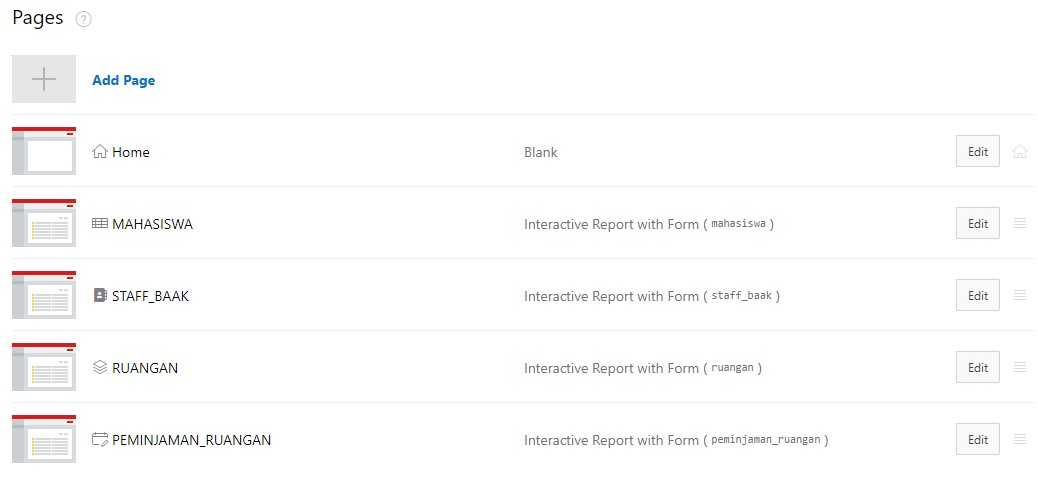
\includegraphics[scale=0.4]{figures/pastikan_page_master_dibuat_terlebih_dahulu.jpg}
        \caption{\textit{Pastikan Page Master Dibuat Terlebih Dahulu}}
        \end{center}
        \end{figure}
        
        \begin{figure}[!htbp]
        \item[15]Setelah sudah pastikan cek dengan lengkap apakah sudah semua
        \begin{center}
        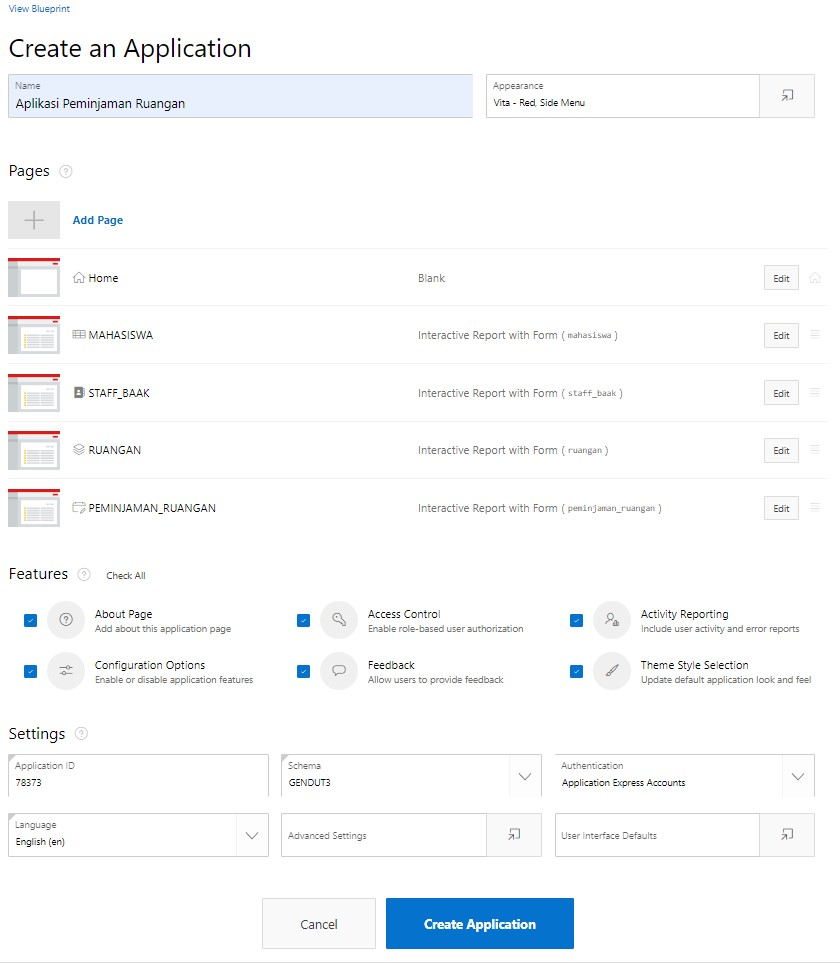
\includegraphics[scale=0.4]{figures/pastikan_sudah_dicek_dan_lengkap.jpg}
        \caption{\textit{Cross Cek Sebelum Di Buat Aplikasi}}
        \end{center}
        \begin{itemize}
            \item Cek kembali semuanya apakah sudah terisi semua dan sudah dicentang semua
        \end{itemize}
        \end{figure}
        
        \begin{figure}[!htbp]
        \item[16]Lalu setelah dirasa sudah klik tombol Create Application
        \begin{center}
        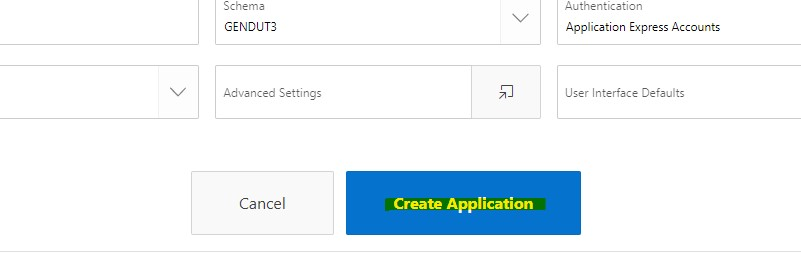
\includegraphics[scale=0.4]{figures/klik_tombol_create_application.jpg}
        \caption{\textit{Klik Create Application}}
        \end{center}   
        \begin{itemize}
            \item CREATE APPLICATION jika anda sudah merasa menggisi semua nya 
        \end{itemize}
        \end{figure}
        
        \begin{figure}[!htbp]
        \item[17]Lalu tunggu loading sejenak untuk proses pembuatan app yang otomatis oleh oracle
        \begin{center}
        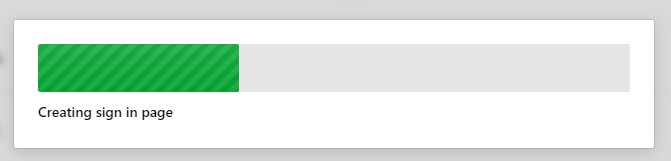
\includegraphics[scale=0.4]{figures/tunggu_loading_app_sdg_dibuat.jpg}
        \caption{\textit{Tunggu Loading App Sedang Dibuat}}
        \end{center}
        \end{figure}
        
        \begin{figure}[!htbp]
        \item[18]Setelah Selesai Anda akan dibawa pada halaman utama Aplikasi anda
        \begin{center}
        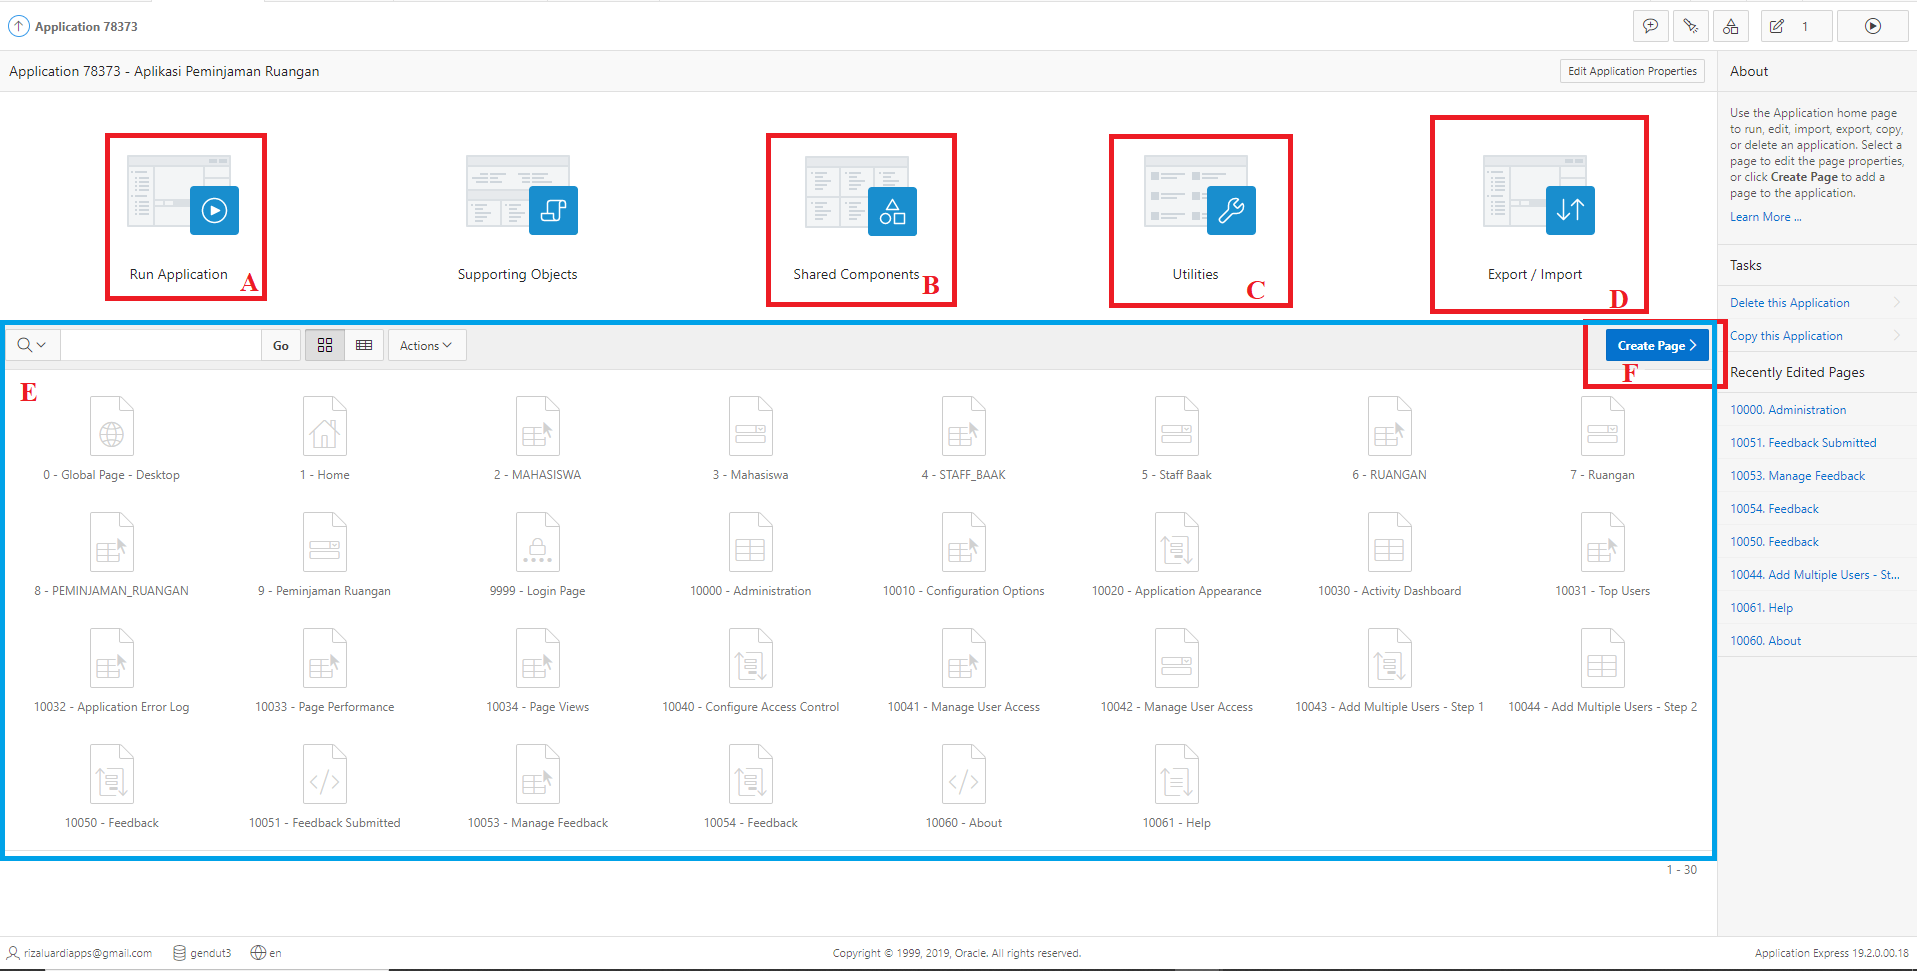
\includegraphics[scale=0.2]{figures/halaman_aplikasi_utiltis.png}
        \caption{\textit{Halaman Utama Apex}}
        \end{center}
        Berikut Penjelasannya
            \begin{itemize}
                \item[A]Untuk Running Aplikasi yang telah dibuat
                \item[B]Shared Components , Berfungsi membuat komponen yang dibutuhkan,nanti yang akan dipakai adalah item list.
                \item[C]Utilities, berfungsi untuk merapihkan halaman tata cara halaman, namun tidak akan dipakai dalam pembuatan aplikasi ini
                \item[D]Export/Import, Berfungsi untuk mengexpor aplikasi menjadikannya sebuah file dan dapat disimpan , lalu untuk memasukkan aplikasi yang telah jadi
                \item[E]Page Aplikasi, berikut adalah Halaman Aplikasi yang telah dibuat tadi sesui urutan pada halaman pertama selalu HOME
                \item[F]Create Page, berfungsi membuat Page Tambahan Pada Aplikasi.
            \end{itemize}
        \end{figure}
        
        \begin{figure}[!htbp]
        \item[19]Pertama kita pilih Run Application, untuk tes aplikasi master yang dibuat tadi, login menggunakan email dan password saat mendaftar
        \begin{center}
        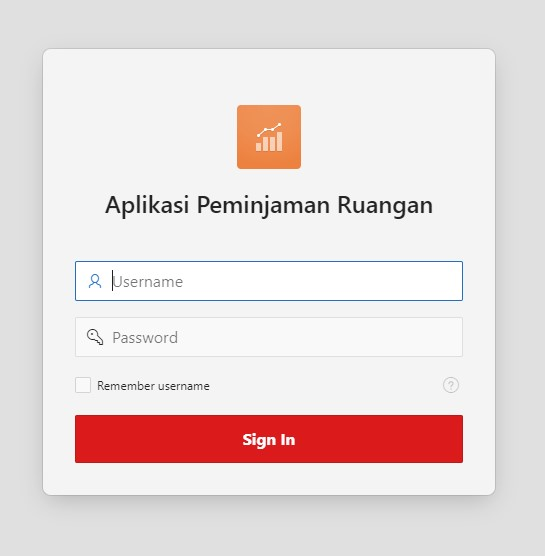
\includegraphics[scale=0.6]{figures/halaman_login_aplikasi.jpg}
        \caption{\textit{Halaman Login Aplikasi}}
        \end{center}
        \end{figure}
        
        \begin{figure}[!htbp]
        \item[20]Berikut adalah tampilan saat di halaman utama Aplikasi
        \begin{center}
        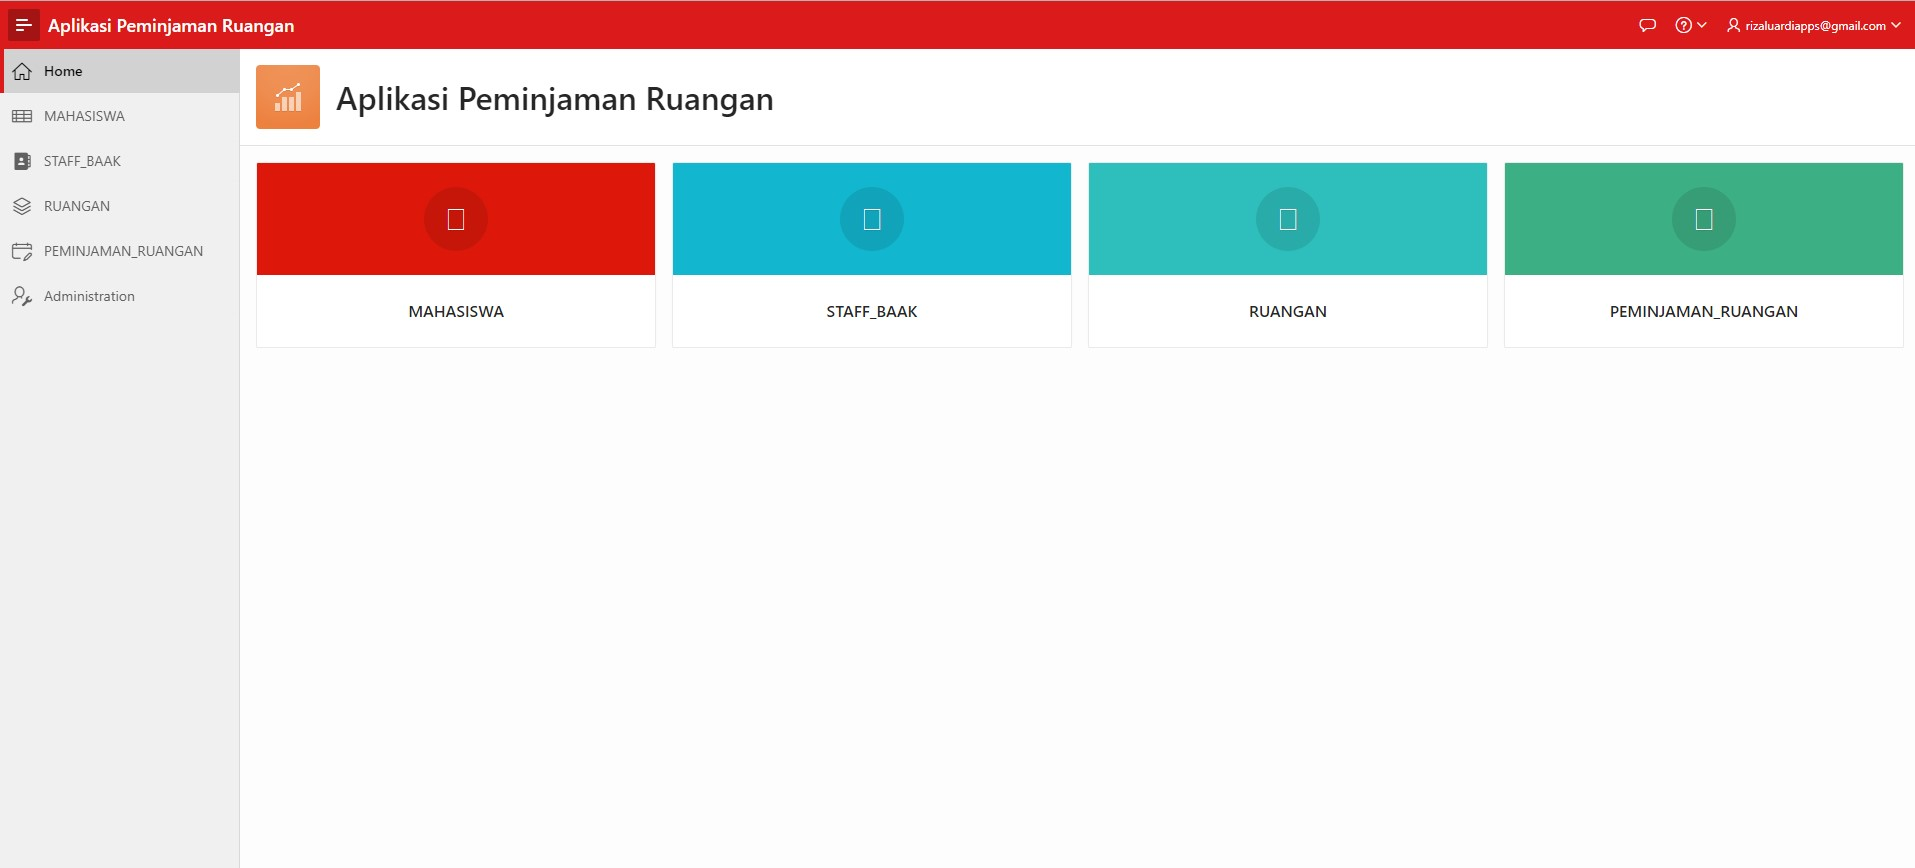
\includegraphics[scale=0.19]{figures/halaman_utm_apps.jpg}
        \caption{\textit{Halaman Utama Aplikasi}}
        \end{center}
        \end{figure}
\end{itemize}
